\icode{E-MD-CA-L3-261112-005}
一长木板\(B\)在水平地面上运动，在\(t = 0\)时其速度为\(v =\) \,\qty{6}{m/s}，此时将一相对于地面静止的物块\(A\)放到木板上。已知物块与木板的质量相等，物块与木板间的动摩擦因数为\(\mu_1 = 0.2\)，木板与地面间的动摩擦因数为\(\mu_2 = 0.1\)，物块与木板间的最大静摩擦力等于滑动摩擦力，且物块始终在木板上。取重力加速度的大小\(g =\) \,\qty{10}{m/s^2}。求：
\begin{enumerate}
	\item 物块刚放到木板上时，物块和木板的加速度大小；
	\item 木板的最短长度\(L\)；
	\item 从\(t = 0\)到木板停止运动，木板位移的大小。
\end{enumerate}
	
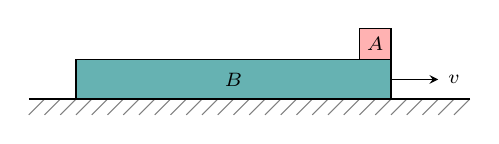
\begin{tikzpicture}[>=stealth,font=\scriptsize]
	\draw[fill=teal!60] (0,0) rectangle(4,.5)node[midway]{\(B\)};
	\draw[fill=red!30] (3.6,.5) rectangle(4,.9)node[midway]{\(A\)};
	\foreach \x in {-.6,-.4,...,5}
		\draw[gray] (\x,-.2)--++(.2,.2);
	\draw[thick] (-.6,0)--(5,0);
	\draw[->] (4,.25)--++(.6,0)node[right]{\(v\)};
\end{tikzpicture}
\begin{answer}
	（1）\qty{2}{m/s^2}\quad\qty{4}{m/s^2}（2）\qty{3}{m}（3）\qty{6}{m}
\end{answer}